\documentclass[border=10pt]{standalone}

\usepackage{tikz}
\usepackage{tikzsymbols}
\usetikzlibrary{calc,patterns,shapes.geometric}

\def\centerarc[#1](#2)(#3:#4:#5){\draw[#1] ($(#2)+({#5*cos(#3)},{#5*sin(#3)})$) arc (#3:#4:#5);}

\begin{document}
	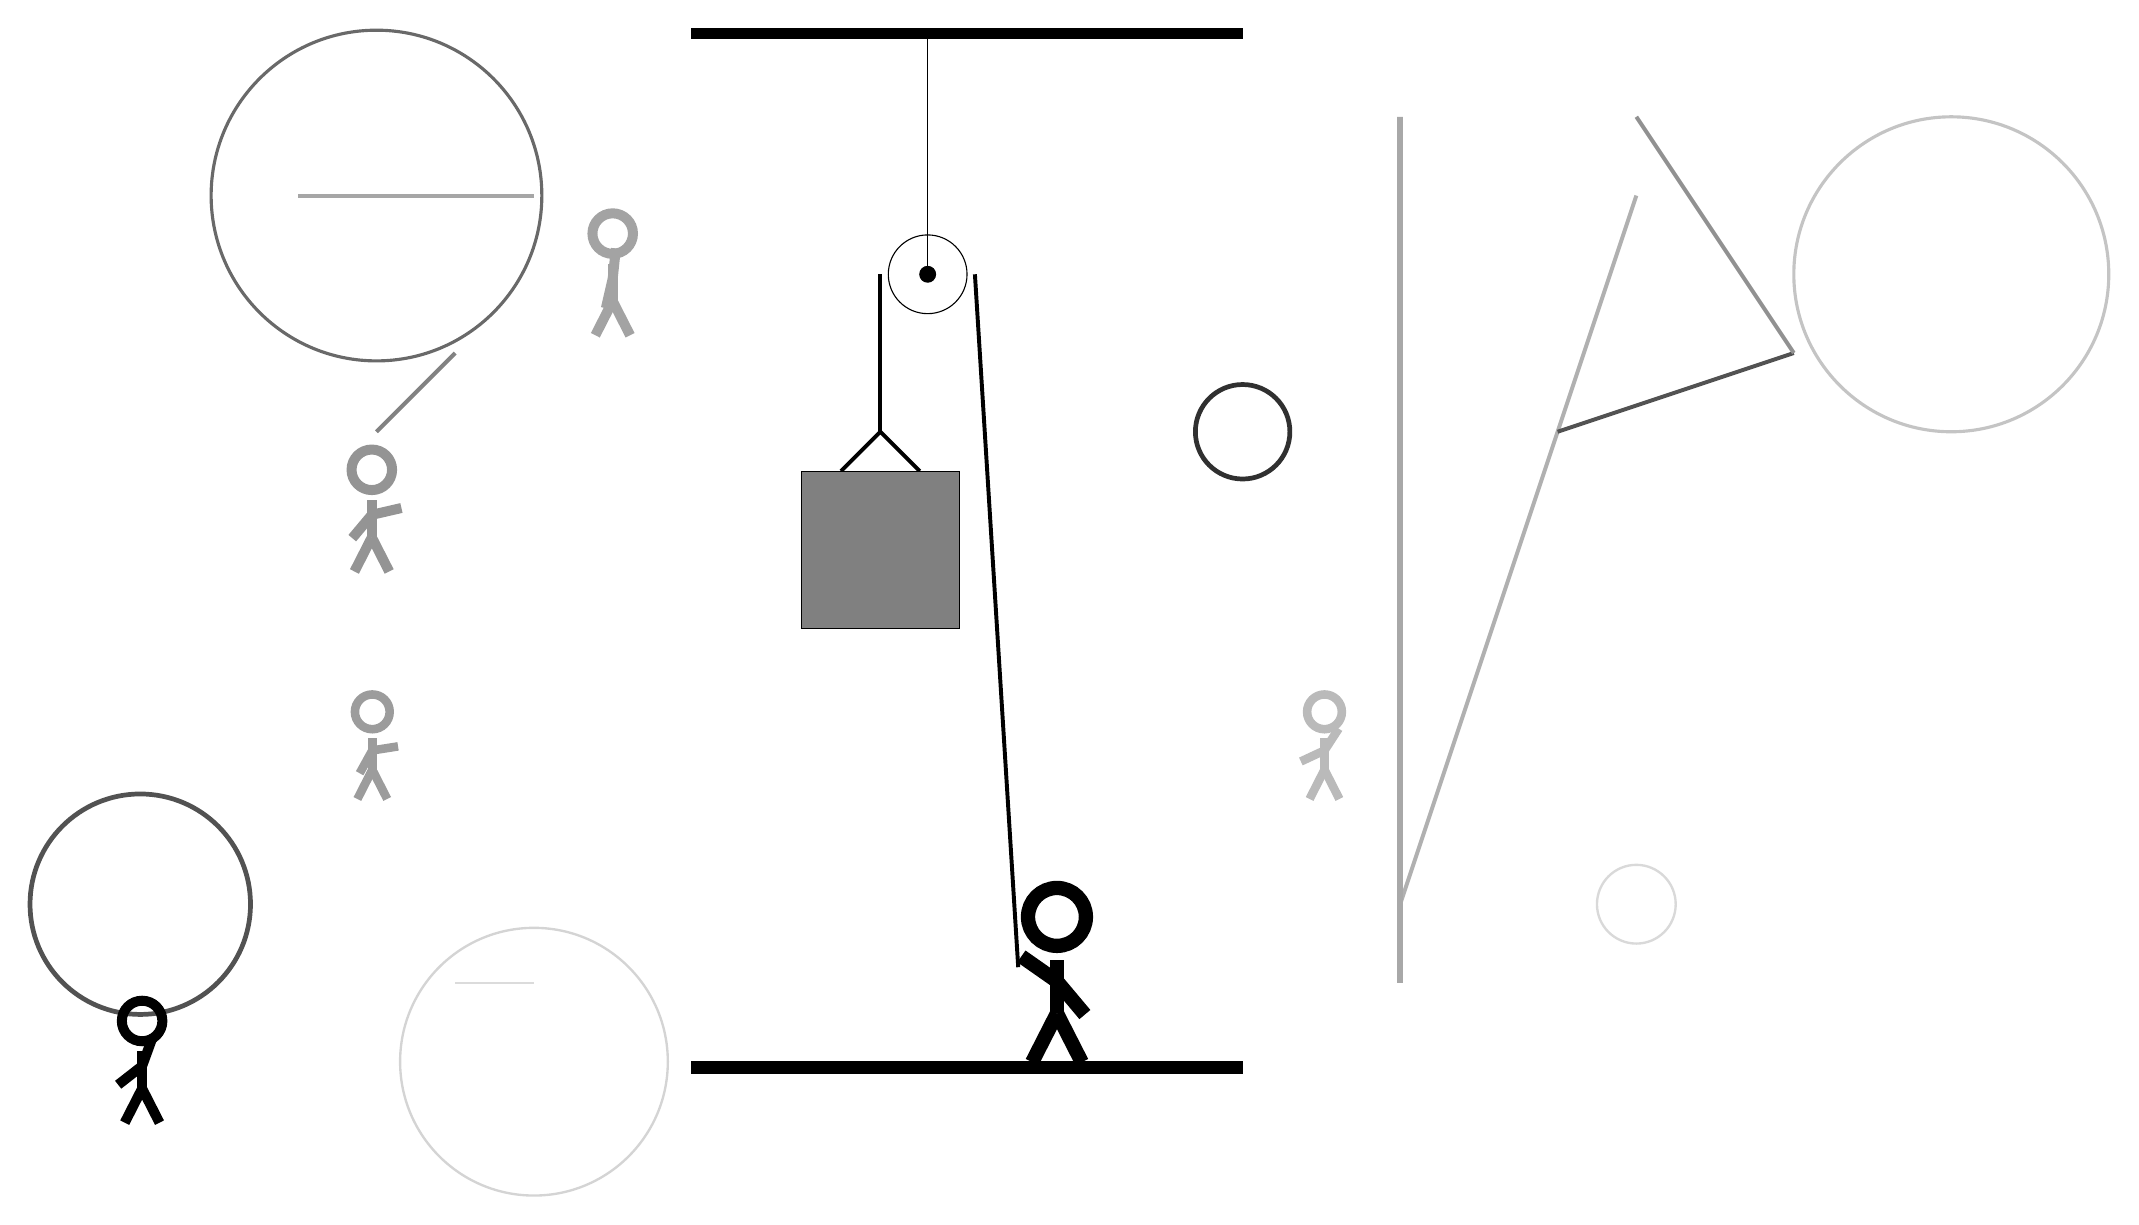
\begin{tikzpicture}
		%%%%% START %%%%%
		
		\draw[fill=black] (-2, 10) rectangle (5, 10.125);
		
		\draw (1, 7) circle (0.5);
		\draw[fill=black] (1, 7) circle (0.1);
		\draw (1, 10) -- (1, 7);
		
		\draw[line width=0.5mm] (-0.1, 4.5) -- (0.4, 5.0) -- (0.9, 4.5);
		\draw[fill=black!50] (-0.6, 4.5) rectangle (1.4, 2.5);
		
		\draw[line width=0.5mm] (0.4, 7) -- (0.4, 5.0);
		\centerarc[line width=0.5mm](1, 7)(0:180:0.6);
		\draw[line width=0.5mm](1.6, 7) -- (2.15, -1.8);
		
		\node at (2.6, -1.9) {\Strichmaxerl[10][-35][-50]};
		
		\draw [line width=0.3mm, color=black!17](-4, -3) circle (1.7);
		
		\draw[line width=0.5mm, color=black!31](7, -1) -- (10, 8);
		\draw [line width=0.4mm, color=black!23](14, 7) circle (2.0);
		\draw[line width=0.7mm, color=black!34] (7, -2) rectangle (7, 9);
		\draw [line width=0.3mm, color=black!15](10, -1) circle (0.5);
		\node[line width=0.4mm, color=black!36] at (-3, 7) {\Strichmaxerl[7][77][84]};
		\draw[line width=0.5mm, color=black!49](-5, 6) -- (-6, 5);
		
		\node[line width=0.4mm, color=black!39] at (-6, 1) {\Strichmaxerl[6][61][9]};
		\draw[line width=0.3mm, color=black!14] (-4, -2) rectangle (-5, -2);
		\node[line width=0.2mm, color=black!42] at (-6, 4) {\Strichmaxerl[7][50][13]};
		\draw[line width=0.5mm, color=black!68](9, 5) -- (12, 6);
		\draw [line width=0.6mm, color=black!81](5, 5) circle (0.6);
		\draw [line width=0.4mm, color=black!59](-6, 8) circle (2.1);
		
		\draw [line width=0.6mm, color=black!68](-9, -1) circle (1.4);
		\draw[line width=0.5mm, color=black!43](10, 9) -- (12, 6);
		\draw[line width=0.5mm, color=black!35](-4, 8) -- (-7, 8);
		
		\node[line width=0.4mm, color=black!27] at (6, 1) {\Strichmaxerl[6][25][57]};
		\node[line width=0.6mm, color=black!100] at (-9, -3) {\Strichmaxerl[7][38][70]};
		
		\draw[fill=black] (-2, -3) rectangle (5, -3.15);
		
		%%%%% END %%%%%
	\end{tikzpicture}
\end{document}